% STATUS: SUPPORT -- c(hbar) -> a / a' / a'' conversion chain (coeff SSOT = calc_correction_functions.m)
% ======================================================
% Compile: xelatex a_gain_chain.tex
% Path:    reference/eq17_analysis/derivation/a_gain_chain.tex
% Wall-effect gain chain, fully expanded in h_bar: the Faxen wall correction
% c(h_bar) -> motion gain a, slope a', curvature a''. z-axis (perpendicular).
% The expanded polynomial coefficients (D, D', D'') are the SSOT from
% model/wall_effect/calc_correction_functions.m. Figure by
% test_script/integration/plot_a_gain_chain.m. Math-only, spacious.
% ======================================================
% fontset=none: no CJK text, do not load Chinese fonts.
\documentclass[12pt,a4paper,fontset=none]{ctexart}

\usepackage[fleqn]{amsmath}
\usepackage{amssymb,bm}
\usepackage{empheq}
\setlength{\mathindent}{0pt}
\usepackage{geometry}
\geometry{margin=2.2cm}
\usepackage{array,booktabs}
\usepackage{graphicx}

\setlength{\parindent}{0pt}
\setlength{\parskip}{0.8em}
\setlength{\abovedisplayskip}{10pt}
\setlength{\belowdisplayskip}{10pt}

\newcommand{\hd}[1]{\par\bigskip\noindent{\large\underline{\textbf{#1}}}\par\nobreak\vspace{1.0ex}}

\begin{document}

\begin{center}
\textbf{\large Wall-effect gain chain:\quad $c(\bar h)\;\to\;a\;\to\;a'\;\to\;a''$}\\[0.4ex]
\small ($z$ axis, perpendicular; \; $\bar h:=h/R$)
\end{center}

\bigskip

\begin{center}
\begin{tabular}{lll}
\toprule
Symbol & Value & Unit \\
\midrule
$R$        & $2.25$                & $\mu$m \\
$\gamma_N$ & $0.0425$              & pN$\cdot$s/$\mu$m \\
$\Delta t$ & $1/1600$              & s \\
$a_{nom}=\Delta t/\gamma_N$ & $1.4706\times10^{-2}$ & $\mu$m/pN \\
\bottomrule
\end{tabular}
\end{center}

\medskip
\[
a':=\frac{da}{dh},\qquad a'':=\frac{d^{2}a}{dh^{2}},\qquad
D:=\frac{1}{c},\qquad
K_h:=\frac{1}{c}\frac{dc}{d\bar h},\qquad
K_h':=\frac{dK_h}{d\bar h}
\]

\hd{1.\quad Wall correction\; $c$}
\[
c(\bar h)=\frac{1}{D(\bar h)},\qquad
D(\bar h)=1-\frac{9}{8\bar h}+\frac{1}{2\bar h^{3}}
-\frac{57}{100\,\bar h^{4}}+\frac{1}{5\bar h^{5}}
+\frac{7}{200\,\bar h^{11}}-\frac{1}{25\,\bar h^{12}}
\]

\hd{2.\quad Gain\; $a$}
\begin{empheq}[box=\fbox]{equation*}
a(\bar h)=\frac{a_{nom}}{c(\bar h)}=a_{nom}\,D(\bar h)
\end{empheq}
\[
a(\bar h)=a_{nom}\!\left[1-\frac{9}{8\bar h}+\frac{1}{2\bar h^{3}}
-\frac{57}{100\,\bar h^{4}}+\frac{1}{5\bar h^{5}}
+\frac{7}{200\,\bar h^{11}}-\frac{1}{25\,\bar h^{12}}\right]
\]

\hd{3.\quad Slope\; $a'$}
\begin{empheq}[box=\fbox]{equation*}
a'(\bar h)=-\frac{a\,K_h}{R}=\frac{a_{nom}}{R}\,D'(\bar h)
\end{empheq}
\[
a'(\bar h)=\frac{a_{nom}}{R}\!\left[\frac{9}{8\bar h^{2}}-\frac{3}{2\bar h^{4}}
+\frac{57}{25\,\bar h^{5}}-\frac{1}{\bar h^{6}}
-\frac{77}{200\,\bar h^{12}}+\frac{12}{25\,\bar h^{13}}\right]
\]

\hd{4.\quad Curvature\; $a''$}
\begin{empheq}[box=\fbox]{equation*}
a''(\bar h)=\frac{a}{R^{2}}\big(K_h^{2}-K_h'\big)=\frac{a_{nom}}{R^{2}}\,D''(\bar h)
\end{empheq}
\[
a''(\bar h)=\frac{a_{nom}}{R^{2}}\!\left[-\frac{9}{4\bar h^{3}}+\frac{6}{\bar h^{5}}
-\frac{57}{5\,\bar h^{6}}+\frac{6}{\bar h^{7}}
+\frac{231}{50\,\bar h^{13}}-\frac{156}{25\,\bar h^{14}}\right]
\]

\hd{5.\quad Curves}
\begin{center}
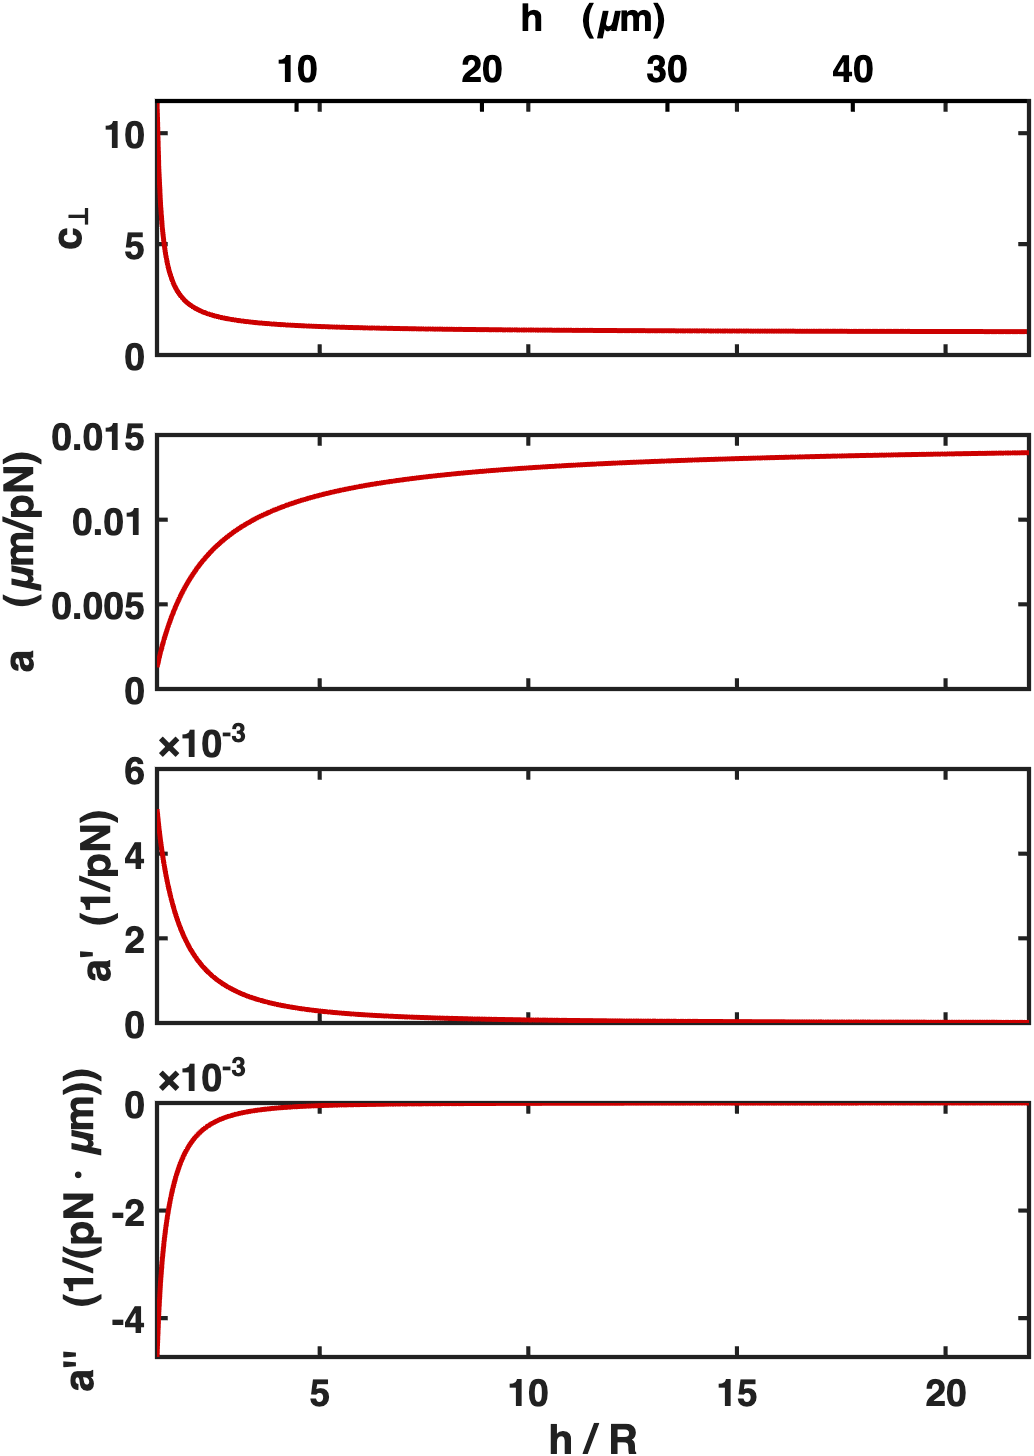
\includegraphics[width=0.66\textwidth]{figures/fig_a_gain_chain_z.png}
\end{center}

\end{document}
